\addcontentsline{toc}{chapter}{QUALITY ASSURANCE AND DEPLOYMENT PIPELINE}
\chapter*{QUALITY ASSURANCE AND DEPLOYMENT PIPELINE}

\section{Overview of Testing Strategy}

The Student Forum application employs a comprehensive testing strategy to ensure code quality, reliability, and security. The testing approach encompasses multiple levels of testing including unit tests, integration tests, and end-to-end tests. This multi-layered testing strategy ensures that individual components function correctly, that they integrate properly with other components, and that the complete user workflows operate as expected.

\subsection{Testing Framework}

The project utilizes Vitest as the primary testing framework. Vitest is a fast and lightweight testing framework that is compatible with Jest's API, making it an excellent choice for Next.js applications. The testing environment is configured with jsdom to simulate a browser environment for DOM-related tests. The configuration is defined in \texttt{vitest.config.ts} and includes settings for global test utilities and module aliasing to match the application's import structure.

\textbf{Configuration Example:}
\begin{verbatim}
import { defineConfig } from 'vitest/config';
import path from 'path';

export default defineConfig({
  test: {
    environment: 'jsdom',
    globals: true,
  },
  resolve: {
    alias: {
      '@': path.resolve(__dirname, './src'),
    },
  },
});
\end{verbatim}

\section{Unit Testing}

Unit tests form the foundation of the testing strategy, focusing on individual functions, components, and modules in isolation. Each unit test verifies that a specific piece of functionality works as expected under various conditions.

\subsection{Security Functions Testing}

The security functions are thoroughly tested to ensure they properly protect against common vulnerabilities. For example, the sanitization functions are tested to verify they effectively prevent XSS attacks:

\textbf{Example Test Case:}
\begin{verbatim}
describe('sanitize', () => {
  it('should strip script tags', () => {
    expect(sanitize('<script>alert(1)</script>')).toBe('');
    expect(sanitize('hello<script>alert(1)</script>world')).toBe(
      'helloworld'
    );
  });

  it('should strip HTML tags', () => {
    expect(sanitize('<div>hello</div>')).toBe('hello');
    expect(sanitize('<img src="x" onerror="alert(1)">')).toBe('');
  });

  it('should handle XSS in img tags', () => {
    const xss = '<img src=x onerror="alert(1)">';
    expect(sanitize(xss)).not.toContain('onerror');
    expect(sanitize(xss)).not.toContain('alert');
  });
});
\end{verbatim}

\textbf{What this test does:} This test suite verifies that the \texttt{sanitize} function properly removes potentially dangerous HTML tags and attributes that could be used for cross-site scripting (XSS) attacks. The first test checks that script tags are completely removed from the input, preventing JavaScript execution. The second test ensures that all HTML tags are stripped, leaving only plain text. The third test specifically targets image tags with event handlers, which are a common vector for XSS attacks. These tests are critical for security as they ensure that user-generated content cannot inject malicious scripts into the application.

\subsection{Validation Functions Testing}

Validation functions are tested to ensure they correctly identify valid and invalid inputs. For example, the UUID validation function is tested with various inputs:

\textbf{Example Test Case:}
\begin{verbatim}
describe('isValidUuid', () => {
  it('should return true for valid UUIDs', () => {
    expect(isValidUuid('550e8400-e29b-41d4-a716-446655440000')).toBe(true);
    expect(isValidUuid('6ba7b810-9dad-11d1-80b4-00c04fd430c8')).toBe(true);
  });

  it('should return false for invalid UUIDs', () => {
    expect(isValidUuid('not-a-uuid')).toBe(false);
    expect(isValidUuid('550e8400-e29b-41d4-a716')).toBe(false);
  });
});
\end{verbatim}

\textbf{What this test does:} This test suite validates that the \texttt{isValidUuid} function correctly identifies properly formatted UUIDs according to the RFC 4122 specification. The first test verifies that valid UUIDs in the correct format (8-4-4-4-12 hexadecimal characters) return true. The second test ensures that malformed UUIDs, non-UUID strings, or incomplete UUIDs return false. This validation is crucial for security and data integrity, as it prevents invalid identifiers from being processed by the system, which could lead to errors or security vulnerabilities.

\subsection{Search Sanitization Testing}

The search sanitization function is tested to ensure it properly handles SQL injection attempts:

\textbf{Example Test Case:}
\begin{verbatim}
describe('sanitizeSearch', () => {
  it('should escape SQL LIKE wildcards', () => {
    expect(sanitizeSearch('100%')).toBe('100\\%');
    expect(sanitizeSearch('test_value')).toBe('test\\_value');
    expect(sanitizeSearch('path\\to\\file')).toBe('path\\\\to\\\\file');
  });

  it('should remove dangerous characters', () => {
    expect(sanitizeSearch("test'injection")).toBe('testinjection');
    expect(sanitizeSearch('test"injection')).toBe('testinjection');
  });
});
\end{verbatim}

\textbf{What this test does:} This test suite ensures that the \texttt{sanitizeSearch} function properly escapes SQL LIKE wildcards (\%, \_) and removes potentially dangerous characters that could be used for SQL injection attacks. The first test verifies that percent signs and underscores (used in SQL LIKE clauses) are properly escaped with backslashes, preventing wildcard matching in database queries. The second test ensures that quote characters (both single and double quotes) are removed, which prevents SQL injection through string termination and concatenation. This is critical for database security, as it prevents malicious users from crafting search queries that could manipulate SQL statements.

\section{Integration Testing}

Integration tests verify that different modules or services work together correctly. These tests ensure that the interfaces between components function as expected and that data flows properly between different parts of the system.

\subsection{Authentication Actions Testing}

Authentication actions are tested to ensure they properly handle various scenarios including successful logins, failed logins, and MFA requirements:

\textbf{Example Test Case:}
\begin{verbatim}
describe('login', () => {
  it('return false success if user cannot be signed in', async () => {
    const mockSupabase = {
      auth: {
        signInWithPassword: vi.fn().mockResolvedValue({
          error: { message: 'error' },
          user: null,
        }),
        mfa: { getAuthenticatorAssuranceLevel: vi.fn() },
      },
    };

    vi.mocked(createClient).mockResolvedValue(mockSupabase as SupabaseClient);

    expect(await login(formState, formData)).toEqual({
      success: false,
      message: 'error',
    });
  });

  it('redirect the valid user to home page if aal level is 1 (no MFA)', async () => {
    const mockSupabase = {
      auth: {
        signInWithPassword: vi.fn().mockResolvedValue({
          error: null,
          user: { id: 'user-1' },
        }),
        mfa: {
          getAuthenticatorAssuranceLevel: vi.fn().mockResolvedValue({
            data: { nextLevel: 'aal1' },
            error: null,
          }),
        },
      },
    };

    vi.mocked(createClient).mockResolvedValue(mockSupabase as SupabaseClient);

    await expect(login(formState, formData)).rejects.toThrow('NEXT_REDIRECT');
    expect(redirect).toBeCalledWith('/');
  });
});
\end{verbatim}

\textbf{What this test does:} These tests verify the authentication flow in different scenarios. The first test simulates a failed login attempt where the Supabase authentication service returns an error. The test ensures that the login function properly handles this error condition by returning a failure state with an appropriate error message. The second test verifies the successful login scenario where the user has an AAL1 (Authentication Assurance Level 1) which means no MFA is required. The test confirms that the user is redirected to the home page ('/') after successful authentication. These tests are essential for security as they ensure that authentication failures are handled gracefully and that successful authentications follow the correct flow.

\subsection{API Route Testing}

API routes are tested to ensure they properly handle requests, validate inputs, and return appropriate responses:

\textbf{Example Test Case:}
\begin{verbatim}
// Example structure for API route testing
describe('API routes', () => {
  it('should handle valid requests correctly', async () => {
    // Mock request and response objects
    const request = new Request('http://localhost/api/example', {
      method: 'POST',
      body: JSON.stringify({ data: 'test' })
    });

    const response = await handler(request);
    expect(response.status).toBe(200);
    expect(await response.json()).toHaveProperty('success', true);
  });

  it('should return appropriate error for invalid inputs', async () => {
    // Test with invalid data
    const request = new Request('http://localhost/api/example', {
      method: 'POST',
      body: JSON.stringify({ invalid: 'data' })
    });

    const response = await handler(request);
    expect(response.status).toBe(400);
  });
});
\end{verbatim}

\textbf{What this test does:} These tests verify that API routes handle both valid and invalid requests appropriately. The first test sends a valid request with proper data and verifies that the API returns a successful response (HTTP 200) with the expected structure. The second test sends invalid data to ensure that the API properly validates inputs and returns an appropriate error response (HTTP 400 Bad Request). These tests are crucial for API security and reliability, ensuring that the application handles both expected and unexpected inputs gracefully.

\section{Test Organization and Structure}

The test suite is well-organized with tests located alongside the code they test or in dedicated test directories. Test files follow naming conventions such as \texttt{*.test.ts} or \texttt{*.spec.ts} to clearly identify test files.

\subsection{Test Categories}

The project includes tests for various components:

\begin{itemize}
    \item \textbf{Security utilities}: Testing sanitization and validation functions to ensure they protect against XSS, SQL injection, and other vulnerabilities
    \item \textbf{Authentication}: Testing login, signup, and MFA flows to ensure secure user authentication and proper error handling
    \item \textbf{API routes}: Testing API endpoints and their responses to ensure proper request handling and security
    \item \textbf{Feature actions}: Testing business logic in feature-specific actions to ensure correct functionality
    \item \textbf{Utility functions}: Testing helper functions and utilities to ensure they behave as expected
\end{itemize}

\subsection{Mocking Strategy}

The testing strategy extensively uses mocking to isolate units of code under test. Dependencies such as Supabase clients, navigation functions, and rate limiters are mocked to ensure tests are predictable and fast.

\textbf{Example Mocking:}
\begin{verbatim}
vi.mock('@/utils/supabase/server', () => ({
  createClient: vi.fn(),
}));

vi.mock('next/navigation', () => ({
  redirect: vi.fn(),
}));
\end{verbatim}

\textbf{What this mocking does:} The mocking strategy allows tests to isolate the functionality being tested by replacing external dependencies with controlled mock objects. The Supabase client mock allows authentication tests to simulate different authentication outcomes without making actual API calls. The navigation mock allows testing of redirect behavior without actually navigating. This approach ensures tests are fast, deterministic, and focused on the specific functionality being tested.

\section{Test Coverage and Quality}

The testing approach emphasizes comprehensive coverage of edge cases, error conditions, and security considerations. Tests are designed to verify both positive and negative scenarios to ensure the application behaves correctly under various conditions.

\subsection{Edge Cases Testing}

Tests include verification of edge cases such as null inputs, malformed data, and boundary conditions:

\textbf{Example Edge Case Test:}
\begin{verbatim}
describe('edge cases', () => {
  it('should return empty string for null/undefined', () => {
    expect(sanitize(null as unknown as string)).toBe('');
    expect(sanitize(undefined as unknown as string)).toBe('');
  });

  it('should preserve whitespace in text', () => {
    expect(sanitize('  hello  ')).toBe('  hello  ');
  });
});
\end{verbatim}

\textbf{What this test does:} This test suite handles edge cases that could cause runtime errors or unexpected behavior. The first test ensures that the sanitize function gracefully handles null or undefined inputs by returning an empty string instead of crashing. This prevents potential runtime errors if the function receives unexpected input types. The second test verifies that the function preserves legitimate whitespace in text, ensuring that normal text formatting is maintained while still removing potentially dangerous content. These tests are important for application stability and user experience.

\subsection{Security Testing}

Special attention is given to security-related tests that verify protection against common vulnerabilities:

\begin{itemize}
    \item Cross-site scripting (XSS) prevention: Tests ensure that user input is properly sanitized to prevent malicious script injection
    \item SQL injection protection: Tests verify that user input is properly escaped to prevent database manipulation
    \item Input validation and sanitization: Tests confirm that all user inputs are validated and sanitized before processing
    \item Authentication and authorization controls: Tests verify that only authorized users can access protected resources
\end{itemize}

\subsection{Security Analysis Tools}

In addition to the comprehensive testing strategy, the project employs automated security analysis tools to identify and address potential vulnerabilities:

\textbf{GitHub Security Analyzer:} GitHub Security Analyzer was configured and used to scan all pull requests targeting the dev branch. During the analysis, it was discovered that the custom text sanitization solution was not fully reliable and could potentially allow security issues. To address this, the decision was made to replace the custom sanitization logic with DOMPurify, a well-established and secure library for sanitizing user-generated content. After applying this change and fixing the reported vulnerabilities, GitHub Security Analyzer confirmed that no critical security issues remained in the project.

\textbf{Dependabot:} Dependabot was configured to continuously monitor the project's dependencies for known security vulnerabilities. The bot automatically scans the project's dependencies and creates pull requests to update vulnerable packages to secure versions. This proactive approach ensures that security patches are applied promptly, reducing the window of exposure to known vulnerabilities. Dependabot also helps maintain the project's security posture by regularly checking for outdated dependencies that may contain unpatched security flaws.

\textbf{OWASP ZAP Security Scanning:} OWASP ZAP was re-run to reassess the overall security status of the application. The scan confirmed that there were no serious or critical vulnerabilities present. Issues related to Content Security Policy (CSP) were resolved, and the remaining minor warnings were evaluated and determined to be non-critical and not harmful to the application's security. The OWASP ZAP scanning process is illustrated in the following figure:

\begin{figure}[h]
\centering
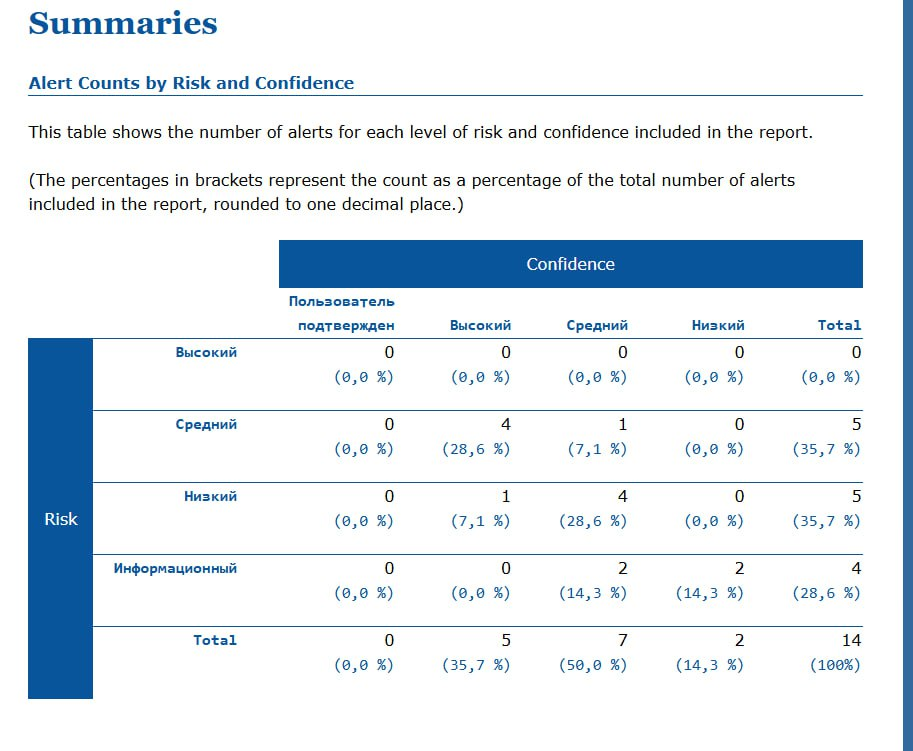
\includegraphics[width=0.8\textwidth]{img/owasp_logs/OWASP.jpg}
\caption{OWASP ZAP Security Scanning Interface}
\label{fig:owasp-zap}
\end{figure}

\section{Logging and Monitoring}

\subsection{Theory of Logging}

Logging is a critical aspect of software development that involves recording events, activities, and states within an application. Logs serve multiple purposes including debugging, monitoring system health, detecting security incidents, and providing insights into application behavior. Effective logging strategies help developers and system administrators understand how an application performs in production environments, identify issues quickly, and maintain system reliability.

Key principles of effective logging include:

\begin{itemize}
    \item \textbf{Log Levels}: Differentiating between debug, info, warning, error, and critical messages to categorize the severity of events
    \item \textbf{Structured Logging}: Using consistent formats that include timestamps, log levels, and contextual information to facilitate analysis
    \item \textbf{Performance Considerations}: Ensuring logging does not significantly impact application performance
    \item \textbf{Security}: Avoiding logging sensitive information such as passwords, tokens, or personal data
    \item \textbf{Retention Policies}: Managing log storage and archival to balance historical data needs with storage costs
\end{itemize}

\subsection{Sentry as Logging Solution}

For the Student Forum application, we implemented Sentry as our primary error tracking and monitoring solution. Sentry is a popular open-source platform that provides real-time error tracking, performance monitoring, and debugging tools for various programming languages and frameworks. It enables developers to capture, aggregate, and analyze errors occurring in production environments, allowing for rapid identification and resolution of issues.

Sentry offers several advantages for our application:

\begin{itemize}
    \item \textbf{Real-time Error Tracking}: Automatically captures and reports errors as they occur in the application
    \item \textbf{Detailed Error Context}: Provides stack traces, user information, and environmental details to help diagnose issues
    \item \textbf{Performance Monitoring}: Tracks application performance metrics and identifies slow operations
    \item \textbf{Release Health}: Monitors the stability of different application releases
    \item \textbf{Alerting System}: Sends notifications when new errors occur or when error rates exceed predefined thresholds
\end{itemize}

The following figures show the Sentry dashboard interface and an example of captured error logs:

\begin{figure}[htbp]
\centering
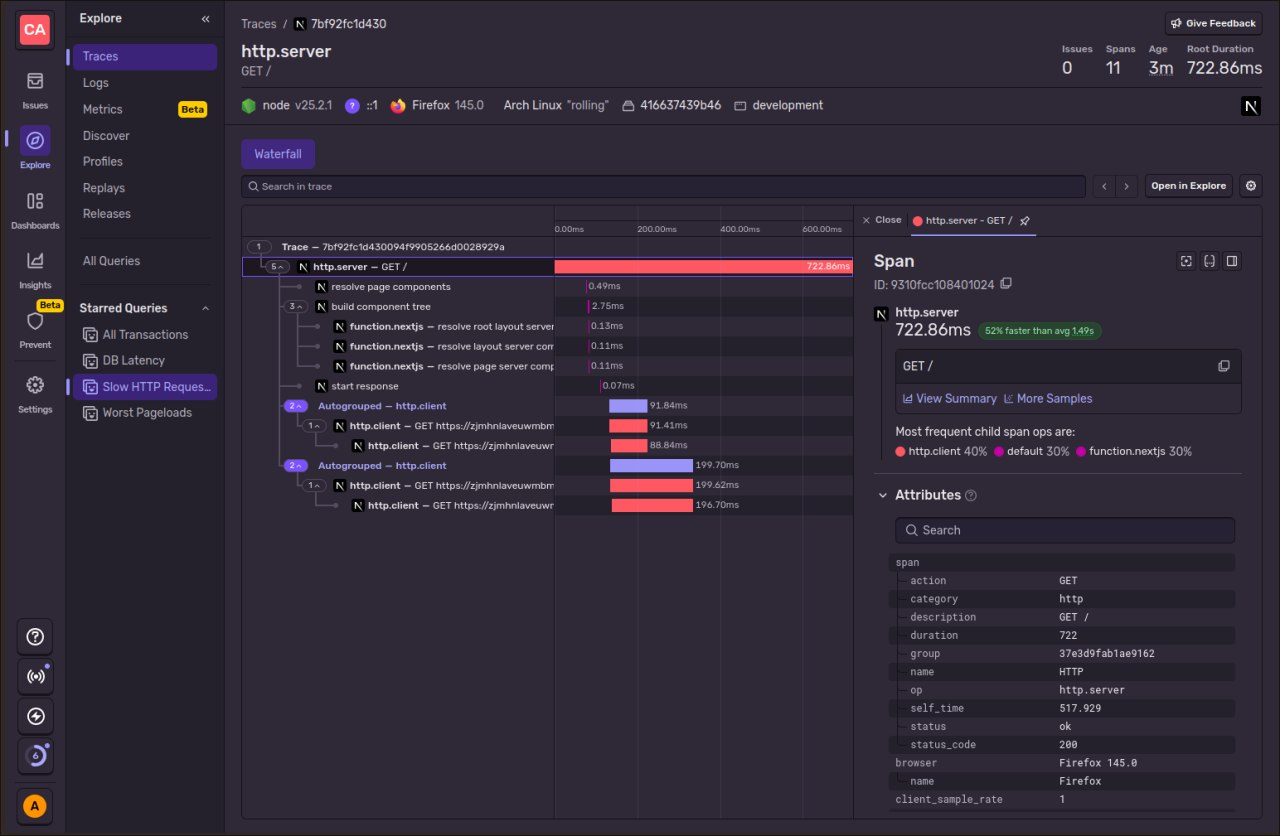
\includegraphics[width=0.6\textwidth]{img/owasp_logs/Sentry.jpg}
\caption{Sentry Dashboard Interface}
\label{fig:sentry-dashboard}
\end{figure}

Figure \ref{fig:sentry-dashboard} illustrates the Sentry dashboard interface, which provides a comprehensive overview of application errors and performance metrics. The dashboard displays key statistics including the number of new issues, event counts, and project activity. It features a clean, intuitive interface that allows developers to quickly identify and prioritize critical issues. The left sidebar contains navigation options for accessing different aspects of error tracking, release health, and performance monitoring. The main panel presents a chronological list of errors, with each issue showing its severity level, title, and the last occurrence timestamp. This centralized view enables development teams to efficiently monitor application health and respond to problems in real-time.

\begin{figure}[htbp]
\centering
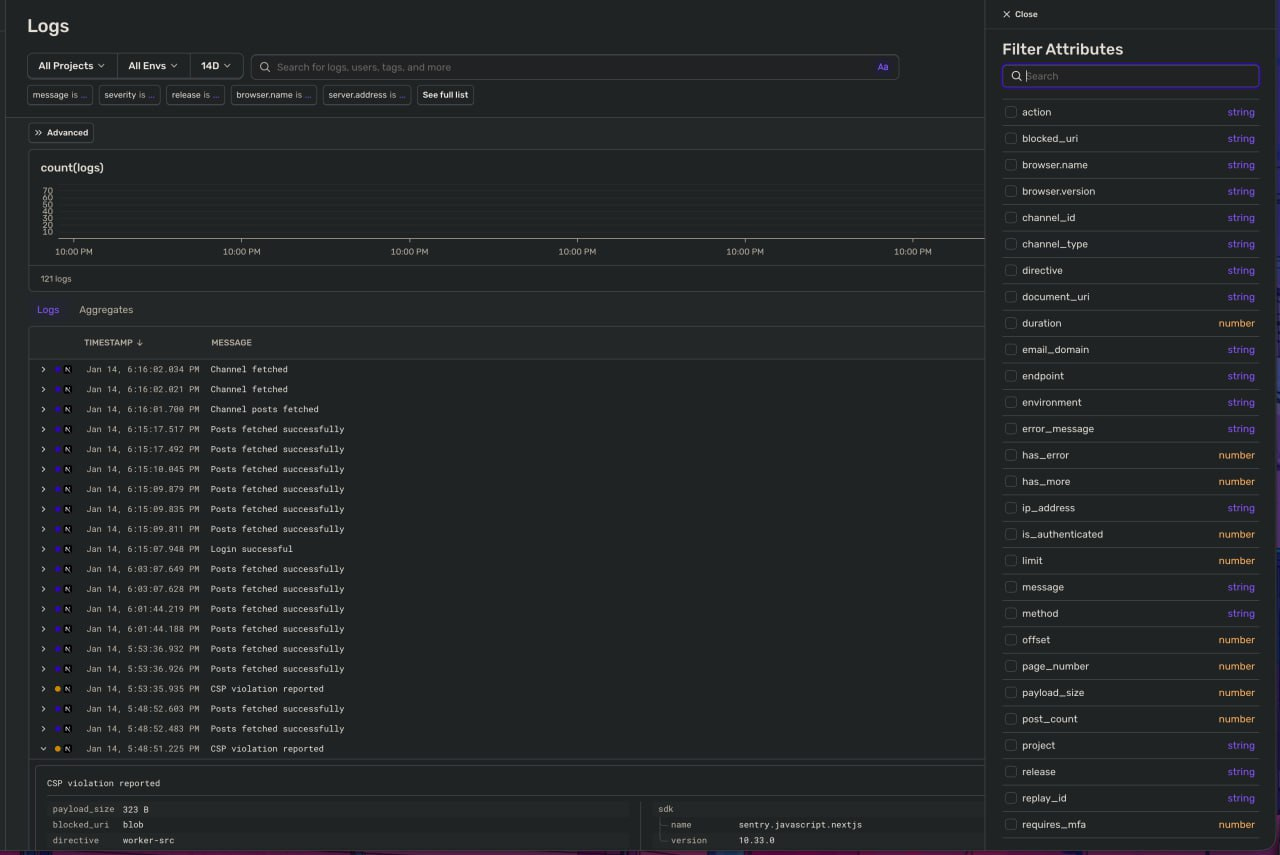
\includegraphics[width=0.6\textwidth]{img/owasp_logs/Sentry_log.jpg}
\caption{Sentry Error Log Example}
\label{fig:sentry-log}
\end{figure}

Figure \ref{fig:sentry-log} displays a detailed view of a specific error captured by Sentry. This interface provides comprehensive information about individual errors, including the complete stack trace, contextual data about the user session, device information, and environmental variables. The error details panel shows the exact location where the error occurred in the code, along with variable values at the time of the exception. Additional tabs provide access to breadcrumbs (preceding events leading to the error), user information, and custom tags that help with categorization and filtering. This granular level of detail enables developers to quickly diagnose and resolve issues by understanding the complete context in which errors occur.

This comprehensive testing approach ensures that the Student Forum application maintains high quality, security, and reliability across all components and user interactions. The tests provide confidence that the application handles both normal and exceptional conditions appropriately, protecting both users and the system from potential vulnerabilities.

\section{Continuous Integration and Deployment (CI/CD)}

\subsection{CI/CD Pipeline Overview}

The Student Forum application implements a robust Continuous Integration and Continuous Deployment (CI/CD) pipeline to automate the process of building, testing, and deploying code changes. The CI/CD pipeline ensures that every code commit undergoes rigorous validation before being deployed to production, maintaining the application's stability and security.

The main deployment pipeline consists of two parallel jobs that must both pass before deployment:
\begin{itemize}
    \item \textbf{Job 1}: Unit tests and linting checks
    \item \textbf{Job 2}: End-to-end tests with Playwright
\end{itemize}

Once both jobs pass successfully, the project is automatically deployed to Vercel. For non-master branches, the deployment occurs in preview mode, while for the master branch, it deploys in production mode.

\subsection{Main Deployment Workflow}

The project utilizes GitHub Actions as the primary CI/CD platform. The main workflow is configured with two parallel jobs that run simultaneously. The first job handles unit tests and linting checks, while the second job runs end-to-end tests with Playwright. The deployment job only executes if both test jobs pass successfully. For the master branch, the application is deployed to Vercel in production mode, while for other branches it's deployed in preview mode.

\subsection{Additional Security Runners}

The project includes additional security-focused runners that complement the main CI/CD pipeline:

\subsubsection{CodeQL Scanning for GitHub Actions}

CodeQL scanning is configured to verify the security of CI/CD files themselves. This runner analyzes the GitHub Actions workflow files to identify potential security vulnerabilities in the automation scripts.

\subsubsection{CodeQL for Source Code}

CodeQL scanning is also configured for the application source code to verify security in pull requests. Additionally, a cron job runs a full security scan on the entire codebase once per week to ensure ongoing security compliance.

This CodeQL workflow provides continuous security analysis of the codebase. It runs on every push and pull request to main, and additionally performs a comprehensive weekly scan of the entire codebase. The workflow analyzes both JavaScript and TypeScript code to identify potential security vulnerabilities, ensuring that security is maintained throughout the development lifecycle.

\subsection{Deployment Strategies}

The application employs several deployment strategies to ensure zero-downtime deployments and quick rollbacks if needed:

\begin{itemize}
    \item \textbf{Vercel Preview Deployments}: For non-master branches, Vercel automatically creates preview deployments with unique URLs for testing
    \item \textbf{Production Deployments}: For the master branch, Vercel deploys to the production environment with automatic SSL certificates and CDN distribution
    \item \textbf{Rollback Mechanisms}: Vercel provides instant rollback capabilities to previous deployments if issues arise
\end{itemize}

\subsection{Deployment Status Checks}

As part of the CI/CD pipeline, GitHub displays a deployment check status when code is pushed to the repository. This provides immediate visual feedback on the status of the automated checks and deployment process. The following figure shows the deployment check status that appears on the GitHub interface when code is pushed:

\begin{figure}[htbp]
\centering
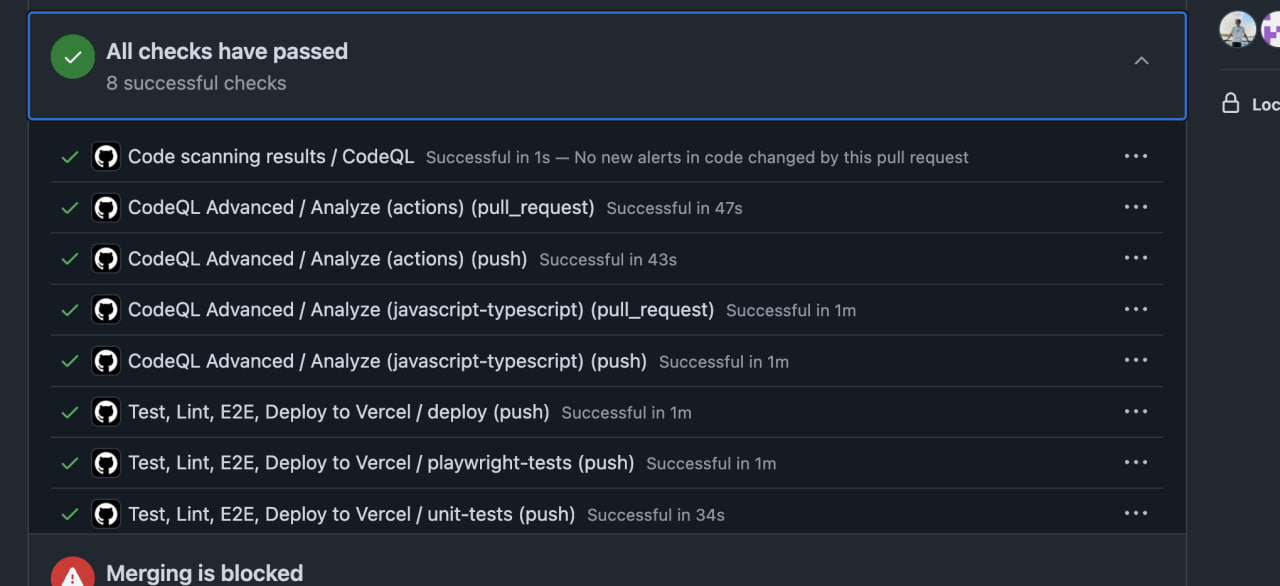
\includegraphics[width=0.8\textwidth]{img/owasp_logs/Deploycheck.jpg}
\caption{GitHub Deployment Check Status}
\label{fig:deploy-check}
\end{figure}

Figure \ref{fig:deploy-check} shows the deployment check status that appears on the GitHub interface when code is pushed. This visual indicator provides immediate feedback on the status of the automated checks, including the parallel unit tests, E2E tests, linting, and security scans. The deployment check ensures that all required validations pass before allowing the merge or deployment to proceed, maintaining the quality and security standards of the Student Forum application.

\subsection{Benefits of the CI/CD Implementation}

The implemented CI/CD pipeline provides several key benefits:

\begin{itemize}
    \item \textbf{Parallel Testing}: Running unit tests and E2E tests in parallel reduces total pipeline execution time
    \item \textbf{Comprehensive Validation}: Both code quality (linting) and functionality (unit and E2E tests) are verified before deployment
    \item \textbf{Automated Security Scanning}: Multiple layers of security checks protect against vulnerabilities
    \item \textbf{Preview Environments}: Automatic preview deployments for non-master branches enable easy testing and review
    \item \textbf{Zero-Downtime Deployments}: Vercel's deployment infrastructure ensures no service interruption during updates
    \item \textbf{Consistent Environments}: Ensures that staging and production environments are identical
    \item \textbf{Visual Status Indicators}: Clear deployment check status on GitHub provides immediate feedback on pipeline health
\end{itemize}

This comprehensive CI/CD implementation ensures that the Student Forum application can be reliably and securely updated with new features and security patches while maintaining high availability and performance for users.